\section{Exercises}
\subsection{Structure}
\noindent
In general, activities are created as follows:
{\em Activities} can be graded directly (e.g. tests).
Alternatively, {\em activities} can also contain unlimited {\em assigments} or {\em checklists}. (However, it is not possible to mix these).
A {\em checklist} may then contain any number of items.
(see the slides in Annex page \pageref{struktur}ff)

\subsection{Creating and Managing Activities}

\begin{figure}[ht]
\begin{center}

\makebox[0pt][l]{
\includegraphics{icon_info}}%
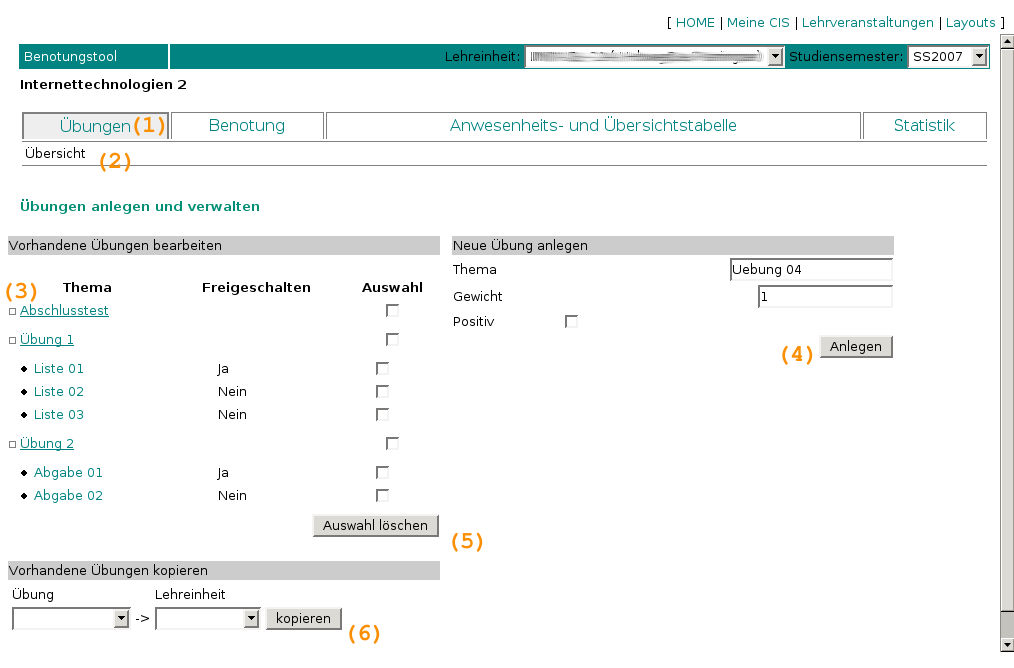
\includegraphics[width=1.0\textwidth]{benotungstool_verwaltung_01.png}

\end{center}
\caption{Activity Management - Overview}\label{verwaltung_01}
\end{figure}

Click on the "'Activities"' tab (see Fig. \ref{verwaltung_01} (1)) - this is also the standard start page.
You can see which level you are currently on within the activity in the subnavigation (2).

The overview page displays all the activities that have been created. 
Clicking the small square in front of the activity name (3) will display all the checklists or assignments in the activity.

Creating a new activity (4): Each activity must be given a name and a point value (for information on how the grades are calculated, see chapter Grading).
If you check the "'Positive"' box, the calculated final grade can only be positive if this activity is completed successfully.

Deleting activities (5): Mark one or more entries to delete them. NOTICE: All the associated data will also be deleted! (sub checklists, assignments, grades already given for the activity, student checklists

Copying activities (6): It is possible to copy an entire activity including all the sub assignments/checklists, as well as all student upload files in other groups of the same course.
Exercises that have been copied once will be synchronized when they are copied again later; i.e. you can adapt an activity in one group and then apply them to the respective activity in another group.\footnote{In future we intend to make it possible to also copy activities from other courses and semesters.}

Clicking on an activity name will open the editing view for the activity. You can edit the activity here, as well as create sub assignments or checklists. It is possible to create either type as long as no other sub elements exist. The first type that you create determines which type can subsequently be used within this activity.

However, once a grade has been given for an activity it will no longer be possible to create any further sub elements. (see chapter \ref{benotung}, page \pageref{benotung}) 

\subsubsection{Assignments}

\begin{figure}[ht]
\begin{center}
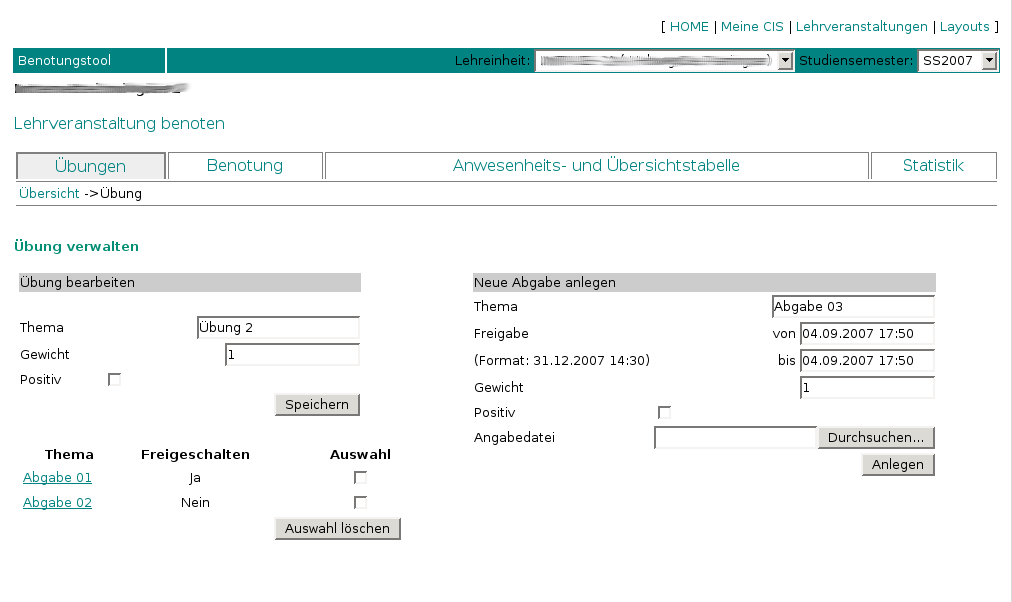
\includegraphics[width=1.0\textwidth]{benotungstool_uebung_detail_abgaben.png}
\end{center}
\caption{Creating Assignments}\label{uebung_detail_abgaben}
\end{figure}

You are in the editing view for an activity (see Fig. \ref{uebung_detail_abgaben}).

To create an assignment you must define the subject, the time by which your student should upload the assignment file, the point value for the assignment within the activity and if it must be completed successfully. In addition, you can also upload an assignment file.\footnote{The file name is automatically generated and assigned to the respective assignment}

Existing assignments can be edited by clicking on the assignment name. (see Fig. \ref{abgabe_detail}). You can change your assignment file here by overwriting it with another assignment or you can delete it by clicking on the [del] link.

\begin{figure}[ht]
\begin{center}
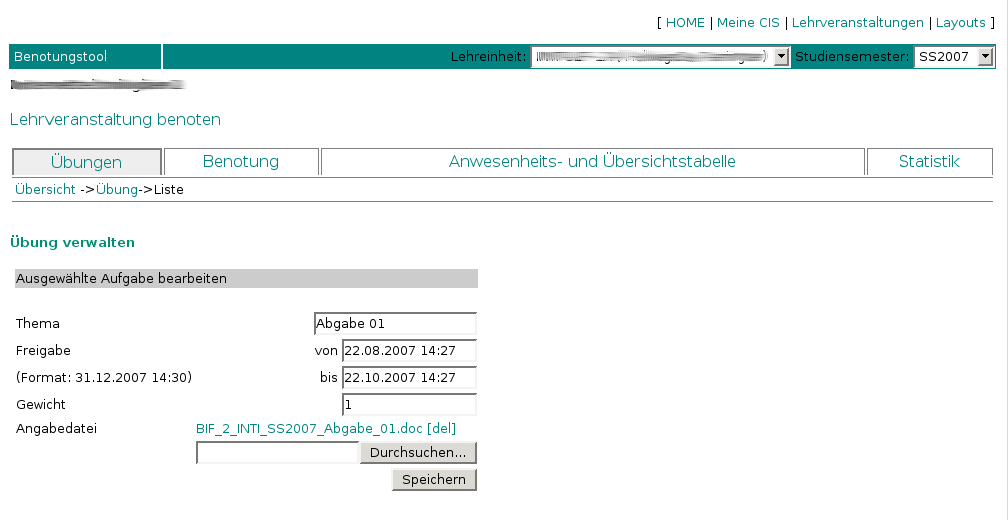
\includegraphics[width=1.0\textwidth]{benotungstool_abgabe_detail.png}
\end{center}
\caption{Editing Assignments}\label{abgabe_detail}
\end{figure}

\subsubsection{Checklists}
\label{kap_kreuzerllisten}

You are in the editing view for an activity (see Fig. \ref{uebung_detail_kreuzerllisten}).

\begin{figure}[ht]
\begin{center}
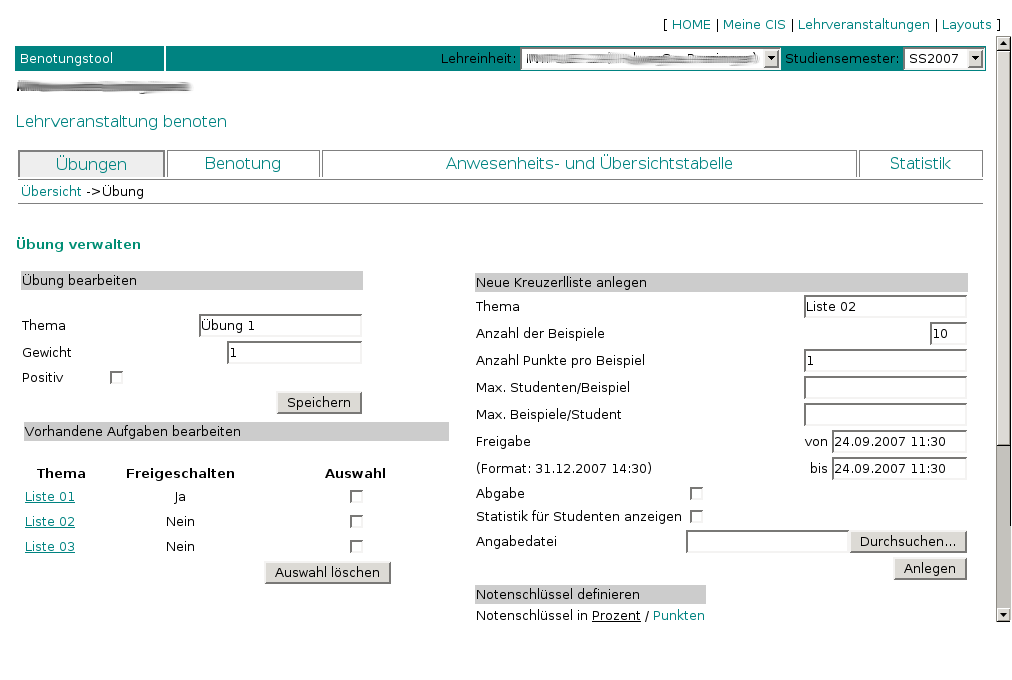
\includegraphics[width=0.9\textwidth]{benotungstool_uebung_detail_kreuzerllisten.png}
\end{center}
\caption{Creating Checklists}\label{uebung_detail_kreuzerllisten}
\end{figure}


To create a checklist you must define the subject, number and point values for the items, the time available for the students to place checkmarks by all the items, as well as whether the statistics for the checkmark distribution should be visible for the students.

If you check the "'Student Uploads"' box, students will be able to upload a file for the checklists. This works the same as an assignment, except that you do not grade these files separately.

In addition, here you can define the maximum number of students who can select a particular item or the maximum number of items that can be selected per student.

Furthermore, you can also upload an assignment file. \footnote{The file name is automatically generated and assigned to the respective checklist}


\begin{figure}[ht]
\begin{center}
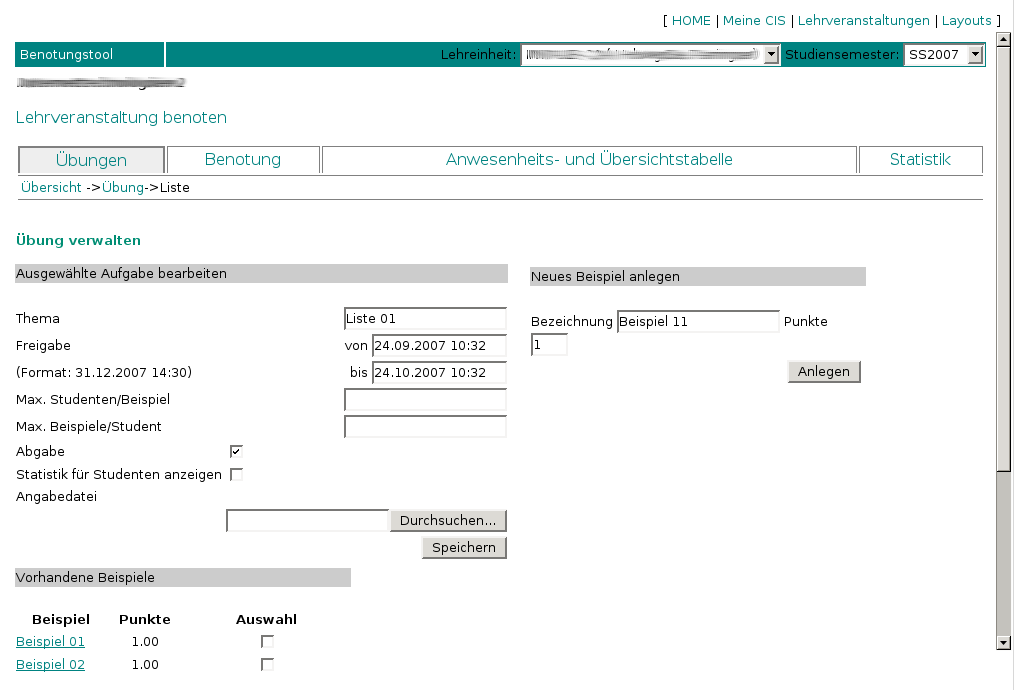
\includegraphics[width=0.9\textwidth]{benotungstool_kreuzerlliste_detail.png}
\end{center}
\caption{Editing Checklists}\label{kreuzerlliste_detail}
\end{figure}

Existing checklists can be edited by clicking on the checklist name. (see Fig. \ref{kreuzerlliste_detail}). You can add, delete or edit items here by clicking on them. You can change your assignment file here by overwriting it with another assignment or you can delete it by clicking on the [del] link.

\subsubsection{Grading Key}
\label{kap_notenschluessel}
The points for all the items for all the checklists within A SINGLE activity are calculated as a grade based on the grading key.
The grading key is defined on the level of the activity that contains the checklists. 

The checklists for this activity will not be included in the automatically calculated grade until a grading key is entered.

You can define the grading key in {\em percentages} or {\em points} (see Fig. \ref{notenschluessel}).

\begin{figure}[ht]
\begin{center}
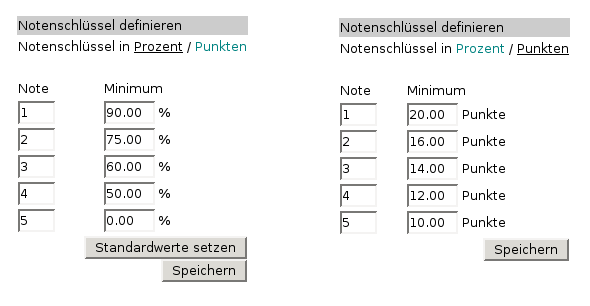
\includegraphics[width=0.8\textwidth]{benotungstool_notenschluessel.png}
\caption{Grading Key in Percentages or Points}\label{notenschluessel}
\end{center}
\end{figure}

You can toggle between the two modes by clicking the respective link. The \underline{underlined mode} is active.

In the {\em percentage} mode you can use the "'Set default values"' button to automatically fill out the fields with the default values.
Adapt the values if necessary, and do not forget to save.
